\documentclass[11pt]{beamer}

\usepackage{epsfig}
\usepackage{amsfonts}
\usepackage{hyperref}
\usepackage[utf8x]{inputenc}
\usepackage{xkeyval}
%\usepackage{default}
\usepackage{../beamer-estat}
\usepackage{amssymb,amsmath,url}

\graphicspath{../}

\title{A presentation on something incredibly interesting}
\subtitle{And something less}
\author{A.~N.~Onymous}
\institute{Methodology; Innovation in official statistics (DG ESTAT)}
\date{\today}

\begin{document}

{
\setbeamercolor{institute}{fg=white}
% The [t] here aligns the title to the top of the slide, otherwise the
% author tends to end up in the picture on the lower right.
\frame[t]{\titlepage} % # 1
}

% ---------------------------------------------------------------------------------
% ---------------------------------------------------------------------------------

\frame { \frametitle{A slide with a dumb title longer than it should reasonably be}
  
  \begin{enumerate}
  \item Item 1
  \item Item 2
  \item Item 3, as interesting as previous items 
  \item the longest item yet, even longer than the one above, though why
    you would want to make it that long is just another matter
  \end{enumerate}
}


% ---------------------------------------------------------------------------------
% ---------------------------------------------------------------------------------

\frame { \frametitle{A slide with images}
  
  \begin{columns}[totalwidth=\textwidth,T]
  \begin{minipage}{0.45\textwidth}
    \begin{column}[t]{\textwidth}
      \centering
      what can we say about \\[0.5cm]
      
\includegraphics[width=\textwidth]{Eurostat_logo.jpg}
    \end{column}
\end{minipage}
  \begin{minipage}{0.45\textwidth}
    \begin{column}[t]{\textwidth}
      \centering
      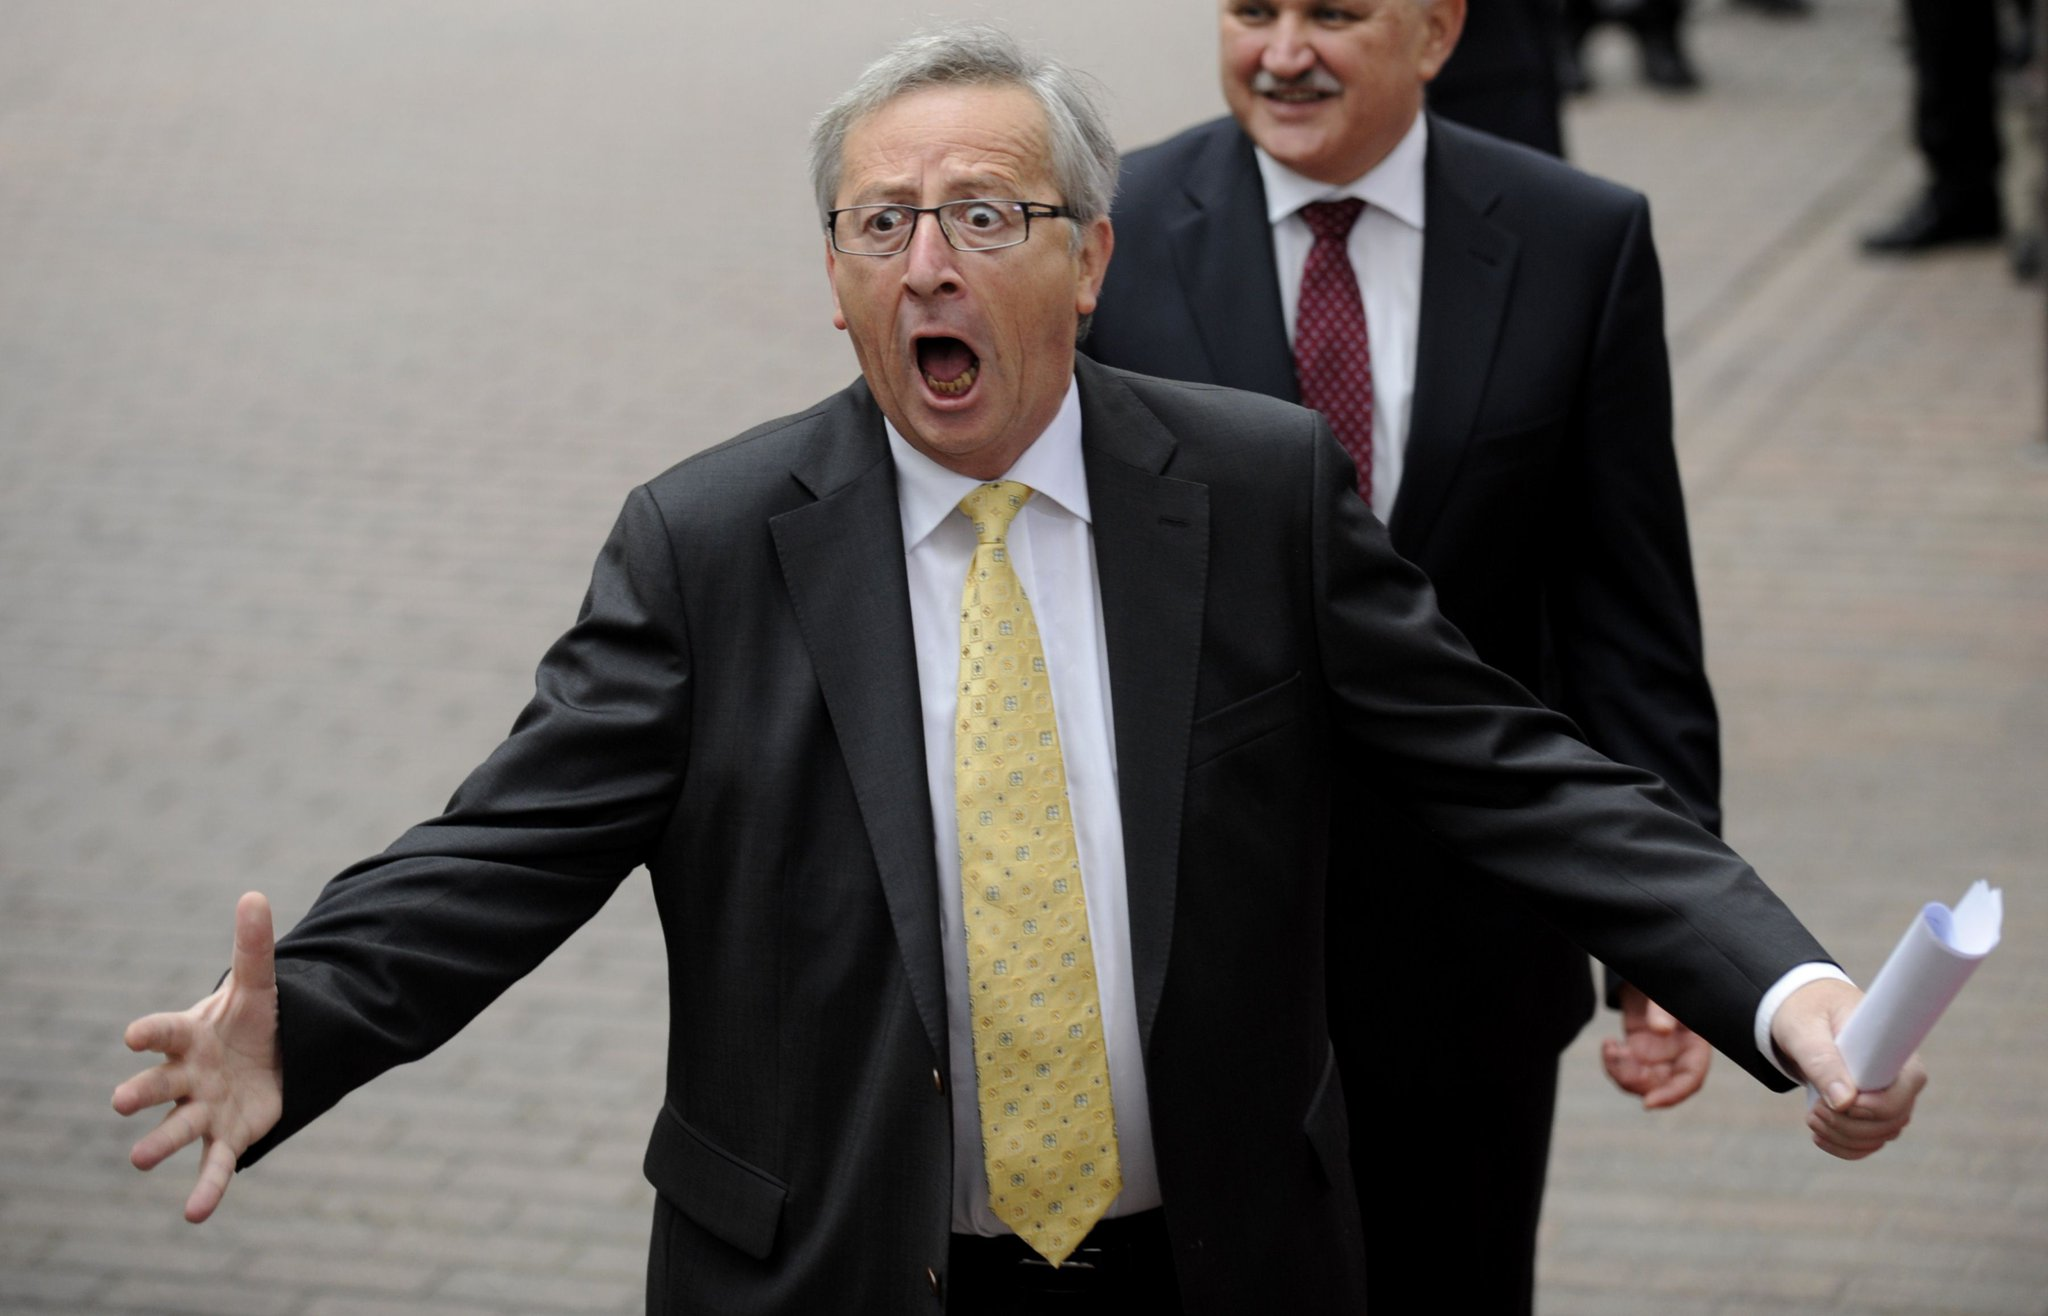
\includegraphics[width=\textwidth]{juncker.jpg}\\[0.5cm]
      amazing... 
    \end{column}
\end{minipage}
  \end{columns}
  
}

% ---------------------------------------------------------------------------------
% ---------------------------------------------------------------------------------
{
\setbeamerfont{normal text}{size=\small}

\frame[c]{ \frametitle{A frame with tasty multifractals}
%% http://www.iacm.forth.gr/papers/grazzini_estimation_cp05.pdf

Let $\epsilon_r(\vec{x})$ be the local dissipation of energy at a point
$\vec{x}$ over a ball $B_r(\vec{x})$  of radius r centered around $\vec{x}$, 
$v_i$  the components of the velocity vector:

    \[
\epsilon_r(\vec{x}) = \frac{1}{\mid B_r(\vec{x})\mid}
\int_{B_r(\vec{x})}
d\vec{x'} \sum_{i,j} [  \delta_i v_j(\vec{x'}) + \delta_j v_i(\vec{x'}) ]
 \]

Under self-similarity assumptions, energy
is transmitted from the larger scales ($L$) to the smaller ones ($r$) by means of an
injection process which  only depends on the
ratio $r/L$, and all the dependence in $r$ of the order-$p$ moment of $\epsilon_r$ 
 is concentrated in the power-law
 \[
\langle \epsilon_r \rangle = \Big[ \frac{r}{L} \Big]^{-\alpha p}  \langle \epsilon^p_L\rangle \propto  r^{\tau_p} 
 \]
}
}
% ---------------------------------------------------------------------------------

\end{document}

